\documentclass[conference]{IEEEtran}
\usepackage[T1]{fontenc}
\usepackage{graphicx}
\usepackage{amsmath}
\usepackage{booktabs}
\usepackage{array}
\usepackage{url}
\usepackage[hidelinks]{hyperref}
\title{A Summary of Digital Image Processing Applications and Suitable Image Features}
\author{\IEEEauthorblockN{Malvino Rosana Pasquale}
\IEEEauthorblockA{Student Number: 25/569865/PA/24015\\Digital Image Processing Course\\Assignment 4}}
\begin{document}
\maketitle
\begin{abstract}
Digital image processing offers practical solutions for extracting information, improving image quality, and supporting visual inspection. This report summarizes five application cases: object counting, scanned-document enhancement, fruit ripeness assessment, surface-defect inspection, and impulse-noise removal. Each case is discussed in terms of its objective, appropriate processing techniques, suitable image features, and practical limitations. Intensity and shape are useful for separating and counting objects; local contrast supports document binarization; color describes visible ripeness changes; texture and edges indicate surface irregularities; and neighborhood statistics help identify impulse noise. The discussion emphasizes that features should be selected according to the physical characteristics of the problem. This is a conceptual review rather than an implementation or experimental evaluation, and no numerical performance claims are made.
\end{abstract}
\begin{IEEEkeywords}
digital image processing, feature selection, segmentation, color, texture, shape
\end{IEEEkeywords}

\section{Introduction}
Digital image processing uses mathematical operations to improve an image or extract useful information from it. An image can be treated as a collection of pixel values, but solving a practical problem requires understanding what those values represent. A dark region could be printed text, a shadow, a damaged surface, or simply an object with a dark color. The same processing operation is therefore not equally suitable for every application.

An image feature is a measurable property that describes a pixel, a neighborhood, or an entire object. Common examples include intensity, color, texture, area, and boundary shape. Features provide a connection between the visual appearance of an image and the information required by a task. Standard image-processing methods include filtering, thresholding, edge detection, morphology, and connected-component analysis~\cite{gonzalez}.

The purpose of this report is to summarize several cases that can be addressed with these techniques and identify suitable features for each case. The discussion focuses on accessible methods appropriate for an introductory course. Proposed workflows explain how a problem could be approached; they do not represent tested systems. The two sample images in Fig.~\ref{fig:samples} are included only to illustrate typical input conditions, not to demonstrate experimental results.

\section{Feature Categories and Selection Principles}
\subsection{Intensity and Color}
Intensity measures brightness and is useful when foreground objects differ from their background. A histogram summarizes the distribution of intensities and can help determine whether threshold-based separation is reasonable. Otsu's method selects a threshold by maximizing between-class variance~\cite{otsu1979}. However, a single threshold can fail when object and background intensities overlap.

Color features describe information that grayscale conversion would remove. Hue and saturation can be useful when the visual difference between categories is mainly chromatic. A color histogram records how frequently different colors occur, while channel means provide a simpler summary. These features are affected by illumination and camera white balance, so consistent acquisition is important.

\subsection{Shape, Texture, and Local Statistics}
Shape features describe the geometry of a segmented region. Area measures region size, perimeter describes boundary length, and aspect ratio distinguishes elongated objects from compact ones. Circularity is commonly expressed as
\begin{equation}
C=\frac{4\pi A}{P^2},
\end{equation}
where $A$ is area and $P$ is perimeter. A continuous circle has circularity equal to one, although pixel sampling affects measured values.

Texture features describe spatial patterns rather than individual pixel values. Local variance indicates intensity variation, while gray-level co-occurrence matrix (GLCM) features characterize relationships between neighboring gray levels. Haralick et al. established a widely used framework for these texture descriptors~\cite{haralick1973}. Local statistics such as the mean and median are also useful for distinguishing isolated outliers from consistent neighborhoods.

\begin{table*}[t]
\caption{Summary of Application Cases, Suitable Features, and Practical Limitations}
\label{tab:summary}
\centering
\footnotesize
\renewcommand{\arraystretch}{1.16}
\begin{tabular}{p{0.14\textwidth}p{0.23\textwidth}p{0.25\textwidth}p{0.27\textwidth}}
\toprule
Case & Candidate techniques & Suitable features & Main limitation\\
\midrule
Object counting & Thresholding, morphology, component labeling & Intensity, area, circularity, centroid & Touching objects, shadows, and scale variation\\
Document enhancement & Background correction, adaptive binarization & Local intensity, contrast, stroke width & Thin strokes and textured backgrounds\\
Fruit ripeness & Color-space conversion, color segmentation & Hue, saturation, color-region ratio, spots & Lighting variation and species dependence\\
Surface inspection & Edge detection, reference comparison, texture analysis & Gradient, elongation, variance, GLCM features & Normal patterns may resemble defects\\
Impulse denoising & Median or switching median filtering & Extreme values, local median deviation & Detail loss and dense corruption\\
\bottomrule
\end{tabular}
\end{table*}

\section{Case I: Counting Separated Objects}
\subsection{Problem Summary and Suitable Techniques}
Object counting is useful in inventory checking, packaging, and classroom examples involving coins or seeds. The objective is to identify each visible object and count it once. Under a simple imaging setup, the objects are separated and placed on a background with a different brightness.

A suitable workflow is grayscale conversion, light smoothing, thresholding, morphological cleanup, and connected-component labeling. Thresholding produces a foreground mask. Morphological operations can remove small fragments and fill small holes. Each remaining connected region is then treated as a candidate object. If objects touch, distance-based watershed segmentation can be considered, but it introduces additional assumptions and parameters.

\subsection{Suitable Features and Their Roles}
\textbf{Intensity} provides the initial separation between object and background. \textbf{Area} helps reject tiny regions that are unlikely to be complete objects. \textbf{Circularity} is useful when the objects are approximately round, as with coins. The \textbf{centroid} records the position of each detected object and helps visualize whether a region corresponds to one physical item.

These features are suitable because counting requires distinct spatial regions, not necessarily object identity. However, area in pixels is not physical size unless the image scale is calibrated. Overlapping objects, shadows, and bright background patches can cause merging or missing detections. A system should therefore be evaluated against manually counted objects across multiple images rather than assuming that every connected region is a valid object.

\begin{figure}[t]
\centering
\begin{minipage}[b]{0.46\columnwidth}
\centering
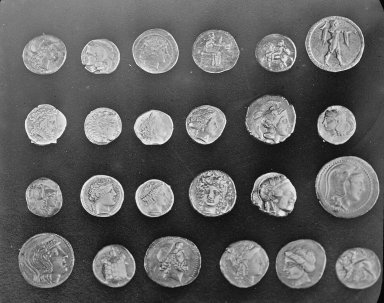
\includegraphics[width=\linewidth]{images/coins.png}\\
\footnotesize (a) Separated coins
\end{minipage}\hfill
\begin{minipage}[b]{0.50\columnwidth}
\centering
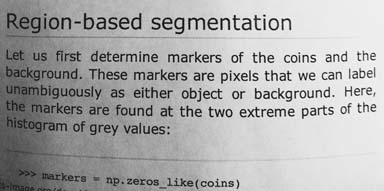
\includegraphics[width=\linewidth]{images/page.png}\\
\footnotesize (b) Scanned text
\end{minipage}
\caption{Illustrative source images from the scikit-image collection~\cite{samples}. The coins illustrate object/background separation; the page illustrates uneven illumination. These are input examples, not processed results.}
\label{fig:samples}
\end{figure}

\section{Case II: Enhancing Scanned Documents}
\subsection{Problem Summary and Suitable Techniques}
Scanned pages and photographs of documents may contain shadows, uneven brightness, and weak contrast. The objective is to separate printed text from the page background so that the document becomes easier to read or prepare for optical character recognition (OCR).

A suitable approach includes grayscale conversion, optional background correction, and binarization. Global thresholding can work with evenly illuminated paper. Adaptive thresholding is more appropriate when background brightness varies because it determines a threshold from each local neighborhood~\cite{thresholds}. Small morphological operations may remove isolated speckles, but aggressive cleanup can erase punctuation or thin strokes.

\subsection{Suitable Features and Their Roles}
\textbf{Local intensity} describes the brightness around a pixel, while \textbf{local contrast} distinguishes dark strokes from nearby paper. \textbf{Stroke width} and \textbf{component area} can help distinguish likely text structures from small isolated noise. \textbf{Edge orientation} or alignment of text lines can also support document deskewing.

Local features are suitable because an illuminated part of a page and a shaded part may require different thresholds. However, connected components do not necessarily correspond to characters: a dot can form a separate component, and neighboring letters can merge. A clean-looking binary page does not establish recognition accuracy. Appropriate evaluation would compare the result with a reference mask or measure character and word errors against a verified transcription.

\section{Case III: Assessing Visible Fruit Ripeness}
\subsection{Problem Summary and Suitable Techniques}
Fruit sorting is a practical agricultural application. For fruits whose skin color changes with ripeness, such as bananas or tomatoes, image processing can support an initial visual assessment. The objective is to group fruit by visible appearance, not to directly measure taste, sugar content, or internal quality.

A basic workflow is to isolate the fruit from the background, convert the image into a suitable color representation, and summarize the colors inside the fruit mask. Hue--saturation--value (HSV) can make chromatic information easier to interpret than raw RGB values. Simple rules may then describe the proportion of green, yellow, or red regions, depending on the fruit species and the intended categories.

\subsection{Suitable Features and Their Roles}
\textbf{Hue distribution} captures dominant skin color, while \textbf{saturation} helps separate vivid skin colors from pale highlights. The \textbf{proportion of color regions} is more informative than a single mean when a fruit has mixed ripeness. \textbf{Dark-spot area} and \textbf{texture variation} may provide additional information about visible blemishes or advanced ripening.

These features match the visible changes being examined, but their interpretation must be species-specific. A green apple is not necessarily unripe, and a shadow is not necessarily a bruise. Glossy reflections, background leakage, and inconsistent lighting can distort color measurements. Controlled illumination and color calibration are therefore important. Any claim about internal ripeness would require independent measurements rather than image appearance alone.

\section{Case IV: Inspecting Surface Defects}
\subsection{Problem Summary and Suitable Techniques}
Manufacturing inspection often aims to locate scratches, cracks, stains, or other irregularities on a surface. Digital image processing can help flag suspicious regions for review, particularly when the normal surface has a consistent appearance.

A suitable workflow includes controlled image acquisition, brightness normalization, edge detection, and texture analysis. An edge detector can emphasize abrupt changes, while comparison with a normal reference image can reveal unexpected structures. Morphological operations can connect nearby crack fragments or remove isolated detections. The result is a candidate defect map rather than an automatic guarantee of product quality.

\subsection{Suitable Features and Their Roles}
\textbf{Gradient magnitude} highlights sharp transitions that may correspond to scratches or cracks. \textbf{Elongation}, \textbf{length}, and \textbf{orientation} help describe narrow linear defects. \textbf{Local variance} and \textbf{GLCM contrast} describe texture changes; \textbf{GLCM homogeneity} describes how strongly neighboring gray levels concentrate near similar values~\cite{haralick1973}.

These features are appropriate because defects often interrupt the expected geometry or texture of the material. However, normal grain, seams, printed patterns, and reflections may also produce strong edges. The normal surface must therefore be characterized before selecting thresholds. Inspection performance should consider both missed defects and false alarms, using independently labeled examples of acceptable and defective surfaces.

\section{Case V: Removing Impulse Noise}
\subsection{Problem Summary and Suitable Techniques}
Impulse noise appears as isolated extreme pixels, often described as salt-and-pepper noise. It can reduce image readability and interfere with later segmentation. The objective is to suppress abnormal pixels while preserving real edges and fine structures.

Median filtering is a suitable introductory method because it replaces a pixel with the median of its neighborhood. Unlike averaging, the median is less influenced by a small number of extreme values. An adaptive or switching approach can instead replace only pixels considered suspicious. Filter size should be chosen carefully because a large neighborhood can remove important details.

\subsection{Suitable Features and Their Roles}
\textbf{Extreme intensity} provides a clue that a pixel may be corrupted. \textbf{Deviation from the local median} indicates whether that pixel disagrees strongly with its surroundings. \textbf{Neighborhood consistency} helps distinguish an isolated outlier from a legitimate bright or dark region. These are restoration cues rather than object-classification features.

An extreme pixel is not automatically noise: a real highlight or a small dark feature can have the same value. Dense corruption can also overwhelm a neighborhood median. Median filtering is especially appropriate for sparse impulses, but it is not universally optimal for all noise distributions. When a clean reference exists, restoration may be evaluated using mean squared error or peak signal-to-noise ratio; these are evaluation metrics, not features available during ordinary processing.

\section{Discussion}
Table~\ref{tab:summary} shows that suitable features depend on the objective. Shape is important when identifying individual objects, but it is less relevant when deciding whether one pixel is corrupted. Color can distinguish visible ripeness changes but contributes little to a grayscale scanned page. Texture can reveal a damaged surface, yet a strongly textured background can make document enhancement more difficult.

Feature selection also depends on acquisition conditions. Region area changes with camera distance, color changes with illumination, and texture descriptors depend on image resolution and neighborhood size. Reliable acquisition and normalization may therefore improve consistency more than adding many unrelated features. Selecting a small set of meaningful features also makes a student-level analysis easier to explain.

Finally, processing techniques, image features, and evaluation metrics should be kept distinct. Thresholding is an operation; intensity is an input property; circularity is a region descriptor; and count error is an evaluation measure. Similarly, a median is a local statistic, while reference-based restoration scores assess the resulting image. A future implementation would require representative images and appropriate reference labels, but this conceptual summary does not claim experimental validation.

\section{Conclusion}
Digital image processing can support a wide range of practical tasks using understandable techniques. Object counting benefits from intensity and geometry, document enhancement from local brightness and contrast, fruit assessment from color, surface inspection from texture and edges, and impulse-noise removal from neighborhood statistics. No single feature is best for all applications. Suitable choices follow the visible characteristics of the target problem and must account for illumination, scale, background, and noise. The five cases demonstrate how to justify feature selection without requiring coding or unsupported numerical results.

\bibliographystyle{IEEEtran}
\bibliography{references}
\end{document}
